\documentclass{kjpaper}
\usepackage[authoryear,sort&compress,round]{natbib}
\bibliographystyle{abbrvnat}
\usetikzlibrary{positioning,fit,arrows.meta,backgrounds,calc}
\usepackage{pifont}
% ---- project macros ----
\newcommand{\sname}{SE-MPPI}
\newcommand{\cmark}{\ding{51}}
\newcommand{\xmark}{\textcolor{gray}{--}}
\DeclareUrlCommand\code{\urlstyle{tt}}
\renewcommand{\UrlBreaks}{\do\/\do\.\do\_\do\-\do\:}
\setlength{\emergencystretch}{2em}
\crefname{section}{Section}{Sections}
\crefname{subsection}{Section}{Sections}
\crefname{appendix}{Appendix}{Appendices}
\crefname{subappendix}{Appendix}{Appendices}
\crefname{table}{Table}{Tables}
\crefname{figure}{Figure}{Figures}
\crefname{equation}{Eq.}{Eqs.}
\creflabelformat{equation}{#2(#1)#3}
\crefname{assumption}{Assumption}{Assumptions}
\crefname{proposition}{Proposition}{Propositions}
\crefname{corollary}{Corollary}{Corollaries}
\crefname{algorithm}{Algorithm}{Algorithms}
\crefname{algocf}{Algorithm}{Algorithms}
\title{\sname: Coordinating Online Local-Minima Escape with Control-Barrier-Function Safety in a Nav2-Native Controller}
\correspondingauthor{kangjmo91@gmail.com}
\paperurl{https://github.com/kjungmo/se-mppi-nav2}
\author[1]{Jungmo Kang}
\affil[1]{Independent Researcher, Seoul, Republic of Korea}
\keywords{model predictive path integral control, control barrier functions, local minima, collision avoidance, ROS~2 Nav2}
\begin{document}
\begin{abstract}
Model Predictive Path Integral (MPPI) control, as shipped in the ROS~2 Nav2 stack, is among the strongest deployable local controllers for mobile robots, yet in narrow, cluttered and dynamic spaces it stalls in local minima and avoids collisions only through soft costs, without a formal safety guarantee. Prior work treats the two weaknesses separately, and none of it ships as a Nav2 controller. In this paper, we introduce \emph{\sname} (Safe-Escape MPPI), a single Nav2-native controller that couples online local-minima detection-and-escape with a control-barrier-function (CBF) safety filter for dynamic obstacles. One entrapment signal switches escape costs into the MPPI rollouts and, through a coordinator, raises the barrier's class-$\mathcal{K}$ gain; we show that forward invariance holds for any positive bounded gain schedule, so an escape admitted by a raised gain stays certified-safe. In a randomized, paired $1{,}200$-trial 2D benchmark built from the controller's primitives, the detection-and-escape layer lifts success from $0\%$ to $88$--$90\%$ on a static U-trap family and from $0\%$ to $62$--$78\%$ on a narrow-dynamic family (Holm-adjusted McNemar $p=1.4\times10^{-9}$ and $1.1\times10^{-6}$), and disabling its free-space gap search returns both families to $0\%$. The escape--safety coordination, by contrast, is statistically indistinguishable from an independent escape+CBF stack; we report this null and claim the coordination as a certified-safe mechanism, not as an empirical gain. The controller also loads and runs in a live ROS~2 Jazzy, Nav2 and Gazebo stack, where it exposed three deployment faults that unit tests could not. Code, raw trials and regeneration scripts: \url{https://github.com/kjungmo/se-mppi-nav2}.
\end{abstract}

\maketitle
\section{Introduction}\label{sec:intro}

\begin{figure}[t]
\centering
\resizebox{\linewidth}{!}{%
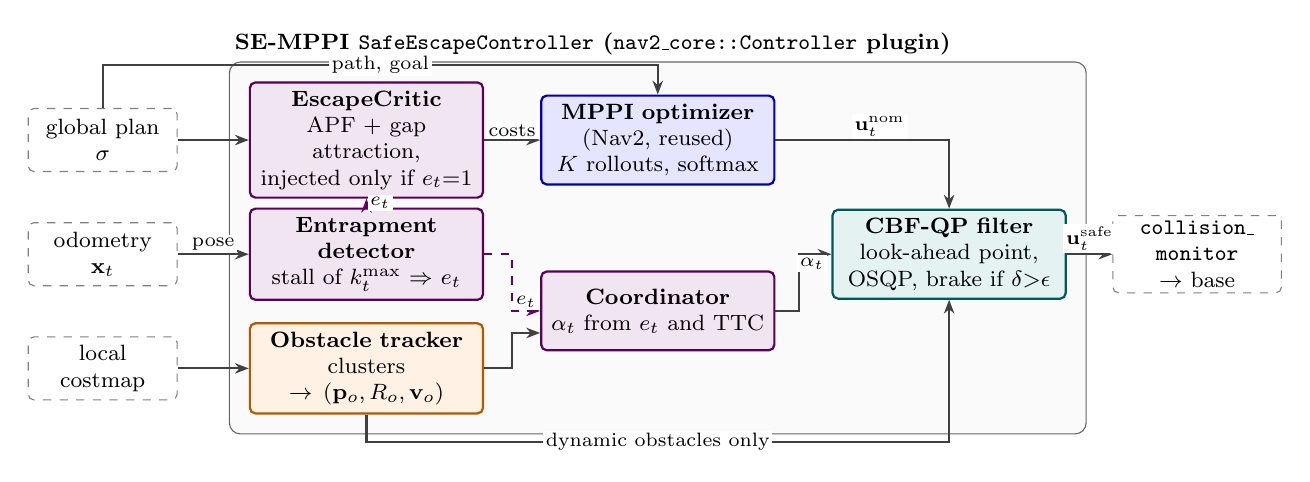
\begin{tikzpicture}[
  font=\footnotesize,
  blk/.style={draw=#1!70!black, fill=#1!10, rounded corners=2pt, thick,
    text width=2.75cm, minimum height=1.0cm, align=center, inner sep=3pt},
  blk/.default=blue,
  io/.style={draw=gray, dashed, rounded corners=2pt, text width=1.75cm,
    minimum height=0.8cm, align=center, inner sep=2pt},
  arr/.style={-{Stealth[length=5pt]}, thick, draw=black!75},
  sig/.style={-{Stealth[length=5pt]}, thick, dashed, draw=violet!80!black},
  lab/.style={font=\scriptsize, fill=white, inner sep=1pt},
]
% inputs
\node[io] (plan) at (0, 1.45) {global plan\\$\sigma$};
\node[io] (odom) at (0, 0) {odometry\\$\mathbf{x}_t$};
\node[io] (cmap) at (0,-1.45) {local\\costmap};
% controller internals
\node[blk=violet] (crit) at (3.35, 1.45) {\textbf{EscapeCritic}\\APF + gap attraction,\\injected only if $e_t{=}1$};
\node[blk] (mppi) at (7.05, 1.45) {\textbf{MPPI optimizer}\\(Nav2, reused)\\$K$ rollouts, softmax};
\node[blk=violet] (det) at (3.35, 0) {\textbf{Entrapment detector}\\stall of $k^{\max}_t$ $\Rightarrow e_t$};
\node[blk=orange] (trk) at (3.35,-1.45) {\textbf{Obstacle tracker}\\clusters $\to(\mathbf{p}_o,R_o,\mathbf{v}_o)$};
\node[blk=violet] (crd) at (7.05,-0.72) {\textbf{Coordinator}\\$\alpha_t$ from $e_t$ and TTC};
\node[blk=teal] (cbf) at (10.75, 0) {\textbf{CBF-QP filter}\\look-ahead point,\\OSQP, brake if $\delta{>}\epsilon$};
\node[io, text width=2.0cm] (cm) at (13.9, 0) {\texttt{collision\_}\\\texttt{monitor} $\to$ base};
% container
\begin{scope}[on background layer]
\node[draw=black!60, fill=black!2, rounded corners=4pt, inner sep=7pt,
  fit=(crit)(mppi)(det)(trk)(crd)(cbf),
  label={[font=\footnotesize\bfseries, anchor=south west, inner sep=2pt]north west:\sname\ \texttt{SafeEscapeController} (\texttt{nav2\_core::Controller} plugin)}] (box) {};
\end{scope}
% edges
\draw[arr] (plan) -- (crit);
\draw[arr] (plan.north) -- ++(0,0.55) -| node[lab, pos=0.25] {path, goal} (mppi.north);
\draw[arr] (odom) -- node[lab, above] {pose} (det);
\draw[arr] (cmap) -- (trk);
\draw[arr] (crit) -- node[lab, above] {costs} (mppi);
\draw[sig] (det) -- node[lab, right] {$e_t$} (crit);
\draw[sig] (det.east) -- ++(0.35,0) |- node[lab, pos=0.75, above] {$e_t$} (crd.west);
\draw[arr] (trk.east) -- ++(0.35,0) |- (crd.west |- 0,-1.0);
\draw[arr] (trk.south) -- ++(0,-0.35) -| node[lab, pos=0.25] {dynamic obstacles only} (cbf.south);
\draw[arr] (mppi.east) -| node[lab, pos=0.3, above] {$\mathbf{u}^{\mathrm{nom}}_t$} (cbf.north);
\draw[arr] (crd.east) -- ++(0.3,0) |- node[lab, pos=0.7, below] {$\alpha_t$} (cbf.west);
\draw[arr] (cbf) -- node[lab, above] {$\mathbf{u}^{\mathrm{safe}}_t$} (cm);
\end{tikzpicture}}
\caption{\textbf{Overview of \sname.} The stock Nav2 MPPI optimizer produces a nominal command from sampled rollouts. A single entrapment signal $e_t$, computed from monotone progress along the global path (\cref{sec:detect}), switches the \texttt{EscapeCritic}'s repulsion and gap-attraction costs into the rollout scoring (\cref{sec:escape}) and tells the coordinator to raise the CBF gain $\alpha_t$ unless a tracked obstacle's time-to-collision is imminent (\cref{sec:coord}). The CBF-QP filter then projects the nominal command onto the barrier-safe set for the tracked dynamic obstacles (\cref{sec:cbf}); Nav2's \texttt{collision\_monitor} remains the last reactive layer.}
\label{fig:overview}
\end{figure}


Autonomous mobile robots increasingly work in cluttered, dynamic indoor spaces such as warehouses, hospitals and service floors, where the local controller must be fast, non-conservative and safe at the same time. Within the ROS~2 Nav2 ecosystem \citep{nav2}, the MPPI controller (\code{nav2_mppi_controller}) is a widely used high-performance option: it samples a batch of control rollouts, scores them with a bank of critic plugins, and fuses them with an information-theoretic softmax \citep{mppi_orig}. With the defaults we build on, it plans over a horizon of $56\times0.05\,\mathrm{s}\approx2.8\,\mathrm{s}$ with $1{,}000$ rollouts per cycle.

Two weaknesses recur in exactly the environments that matter most. First, \emph{local-minima entrapment}: a finite horizon and zero-mean Gaussian sampling make the robot stall or oscillate in front of non-convex obstacles. Within the MPPI critic set, Nav2's mitigations (\code{PreferForwardCritic}, \code{TwirlingCritic}) are always-on cost shaping that neither detects entrapment nor steers an escape. At the stack level, Nav2 does detect a stall: the controller server's progress checker reports a failure when the robot has not moved a set distance within a set time, and the default behaviour tree then clears the costmaps and runs generic recoveries such as spinning, waiting and backing up \citep{nav2,nav2_progress,nav2_bt}. These recoveries are not directed toward an opening. In the MPPI literature, escape methods either reshape the sampling distribution all the time \citep{log_mppi,tsallis_mppi,svg_mppi,biased_mppi,flow_mppi} or add guidance: GP-MPPI recommends a free-space subgoal from a learned navigability surface \citep{gp_mppi}, and repulsive-potential augmentation adds an artificial potential field to the MPPI cost \citep{drpa_sii}, which DRPA-MPPI switches on only when it detects entrapment \citep{drpa_mppi}. None of these carries a safety certificate.

Second, \emph{no formal safety}: in Nav2 MPPI, collision avoidance is encoded as soft costs, the costmap is a present-time snapshot with no prediction of obstacle motion, and \code{collision_monitor} is purely reactive. CBF--MPPI fusions supply safety \citep{shield_mppi,br_mppi,scbf_mppi,dualguard,gs_mppi}, but none of them detects entrapment or adds an escape mechanism (GS-MPPI counters the myopic behaviour often associated with CBFs through long-term performance terms), and none ships as a Nav2 controller. Among CBF integrations with Nav2 that we could verify, the Nav2 documentation describes inserting a third-party product, the 3Laws Supervisor, which its vendor describes as based on CBFs, into the command chain after the controller \citep{nav2_3laws,threelaws_pr}; it is a separate node rather than a controller plugin, and neither source describes a mechanism for escaping local minima.

The two weaknesses also interact: conservatism for safety invites entrapment, and aggressive escape invites collision. Several works outside Nav2 and MPPI address both at once, among them model predictive control that escapes local minima while keeping a safe backup trajectory \citep{soloperto}, gap-based local planners with provable collision-free properties \citep{potential_gap,safer_gap,dynamic_gap}, and modulated CBF filters \citep{mcbf_qp} that reduce or eliminate, among moving obstacles, the spurious equilibria that CBF quadratic programs (QPs) can introduce \citep{reis_cbf_equilibria}, with concurrent extensions \citep{xue_proactive,chen_milp_cbf}.

We present \emph{\sname}, a Nav2 controller plugin that subclasses the stock MPPI controller and post-processes its command each cycle (\cref{fig:overview}). A single entrapment detector, driven by monotone progress along the global path and running inside the controller rather than at the stack level, is the one source of truth for the whole controller. When it fires, an \code{EscapeCritic} switches repulsion and free-space gap-attraction costs into the rollout scoring, and a coordinator raises the gain of a look-ahead-point CBF filter so that the escape manoeuvre is admitted, unless a tracked obstacle's time-to-collision is imminent. This is a system contribution, and we state it as such:
\begin{itemize}
    \item \emph{A Nav2 Controller Integrating Escape and CBF Safety}: a public Nav2 local-controller plugin that combines online local-minima detection-and-escape with a CBF safety filter for tracked dynamic obstacles, packaged as a \code{nav2_core::Controller} plus a pluginlib MPPI critic over a plugin-free core, and released under Apache-2.0. Each ingredient has precedent: gated repulsion in DRPA-MPPI \citep{drpa_mppi}, free-space subgoal and gap guidance in GP-MPPI \citep{gp_mppi} and gap-based planners \citep{potential_gap,safer_gap}, CBF filtering of MPPI commands \citep{scbf_mppi}, and a supervisor for Nav2 that its vendor describes as CBF-based \citep{nav2_3laws,threelaws_pr}. What is new is their integration inside one Nav2 controller; to our knowledge no public controller plugin already provides it.
    \item \emph{An Entrapment-Gated Gain Schedule}: a rule that raises the CBF class-$\mathcal{K}$ gain on detected entrapment and drops it back on an imminent time-to-collision. Online adaptation of CBF gains is established, including selecting class-$\mathcal{K}$ parameters to reduce predicted deadlock \citep{kim_adaptive_cbf} and letting MPPI optimize a barrier-rate parameter \citep{br_mppi}; our rule is a simpler, rule-based two-level instance of online gain adaptation whose specific elements are its trigger and its time-to-collision override. Its invariance property (\cref{prop:invariance}) is a known result for time-varying class-$\mathcal{K}$ terms \citep{ada_cbf,rt_cbf}, which we restate as a conditional lemma: it covers the look-ahead point and the tracked dynamic obstacles, assumes the barrier inequality holds between samples, and requires a slack-free QP. In our benchmark the schedule is empirically indistinguishable from an independent escape+CBF stack.
    \item \emph{Paired Benchmark and Deployment Evidence}: a randomized, seed-deterministic $1{,}200$-trial benchmark on a Python 2D mirror of the controller's primitives ($200$ seeded worlds, each run under six configurations) with paired McNemar tests and Holm correction, every number regenerated from committed per-trial data, together with a live ROS~2 Jazzy, Nav2 and Gazebo integration that exposed three faults unreachable from unit tests.
\end{itemize}

We are deliberately conservative about novelty and about what we claim empirically. Fusing CBFs with MPPI is not new, and neither is gated escape, online adaptation of the CBF gain, or treating escape and safety together; the paper is best read as a system report on putting these pieces into one Nav2 controller. The measured win, in the 2D mirror, is the online detection-and-escape layer: success rises from $0\%$ to $88$--$90\%$ on the static U-trap family and from $0\%$ to $62$--$78\%$ on the narrow-dynamic family, and the gap search is load-bearing, since without it both families stay at $0\%$ (\cref{sec:results,sec:ablation}). In the mirror the gap acts as a temporary subgoal, close to the subgoal guidance of GP-MPPI \citep{gp_mppi}; the gap cost of the C++ critic has not been ablated. The coordination has the conditional invariance property of \cref{prop:invariance} yet produces no measurable outcome difference in the regimes we could test, and we delimit where it should matter (\cref{sec:discussion}). The remaining claims are Nav2-native deployment and the faults a live stack exposes; no live run has yet reached its goal, and no stack-level or third-party baseline has been run (\cref{sec:discussion}).

\section{Related Work}\label{sec:related}

\noindent\textbf{MPPI and Deployable Local Controllers.} Nav2 MPPI \citep{nav2,mppi_orig}, TEB \citep{teb}, DWB, a Nav2 planner of the dynamic-window family \citep{dwa}, and Regulated Pure Pursuit \citep{rpp} are the standard deployable local controllers. MPPI's critic interface (\code{mppi::critics::CriticFunction}) exposes the per-rollout trajectories, the reference path, the goal and the furthest-reached path index, which are exactly the signals needed for entrapment detection, so a custom critic can be inserted without forking the optimizer. \sname{} uses this interface for escape and adds an output-side safety filter, instead of replacing the optimizer. Around the controller, Nav2 already handles stalls at the stack level: the controller server runs a progress checker, by default \code{SimpleProgressChecker}, which reports a failure when the robot has not moved a set radius within a set time allowance, and the default behaviour tree answers with costmap clearing, spinning, waiting and backing up \citep{nav2_progress,nav2_bt}. \sname's detector differs in that it runs inside the controller on progress along the path and steers the escape instead of triggering generic recoveries; the two mechanisms can coexist.

\noindent\textbf{Local-Minima Escape.} Most escape methods for MPPI are always-on changes of the sampling distribution: log-MPPI \citep{log_mppi}, Tsallis-divergence MPC \citep{tsallis_mppi}, Stein-variational guidance \citep{svg_mppi}, ancillary-controller biasing \citep{biased_mppi}, and learned sampling distributions \citep{flow_mppi}. Others add guidance. GP-MPPI learns a sparse-Gaussian-process model of the navigable space around the robot and recommends a free-space subgoal to the local MPPI planner, which lets the robot escape local minima without a global map \citep{gp_mppi}. Fuke et al.\ add a repulsive artificial potential to MPPI to avoid local minima without global path guidance \citep{drpa_sii}, and their DRPA-MPPI detects potential entrapment on the predicted trajectories and only then switches to a cost with repulsion away from the local minimum \citep{drpa_mppi}. DRPA-MPPI is the closest detect-and-switch method and GP-MPPI the closest subgoal method; neither has a CBF or other formal safety layer, and neither is Nav2-integrated. \sname{} combines both ideas in a simpler form, a path-progress stall detector gating a classical repulsive potential \citep{khatib_apf} and a ray-cast gap bearing, and its safety filter runs alongside the escape rather than gating it. Gap-based local planners are closer still to the overall architecture. Potential Gap combines gap-based local navigation with artificial potential fields and restores provable collision-free properties for realistic robot models \citep{potential_gap}; Safer Gap adds nonlinear model predictive control with keyhole zeroing-barrier-function constraints and a point-wise optimization-based safety filter as the final layer \citep{safer_gap}; and Dynamic Gap extends provably collision-free gap-based navigation to dynamic environments by modelling how gaps evolve over time \citep{dynamic_gap}. Relative to this line, \sname{} uses a gap only as a gated escape heuristic inside MPPI, and its barrier covers only tracked dynamic obstacles.

\noindent\textbf{Escape and Safety Together.} Several works treat entrapment and safety jointly. Soloperto et al.\ optimize an exploration trajectory together with a safe backup trajectory in a model predictive controller and prove convergence, feasibility and constraint satisfaction under partially unknown constraints \citep{soloperto}. The modulated CBF-QP of Xue and Figueroa reduces or eliminates, in dynamic environments, the spurious equilibria that CBF-QP filters create \citep{reis_cbf_equilibria}, and was tested on Ridgeback and Fetch robots \citep{mcbf_qp}. Concurrent work adds learned predictive barriers for moving concave obstacles to this filter \citep{xue_proactive}, and pairs a mixed-integer MPC planner with a Minkowski-difference CBF filter to mitigate the local-minimum behaviour of reactive CBF navigation in U-shaped and maze-like environments \citep{chen_milp_cbf}. These methods mitigate or avoid minima inside the planner or the barrier itself, whereas \sname{} leaves the barrier unchanged and escapes through the MPPI cost. None of them is packaged as a Nav2 controller.

\noindent\textbf{CBF--MPPI Safety.} Three fusion styles exist as research code: CBF conditions in the rollout cost or the sampling (Shield-MPPI \citep{shield_mppi}, which adds a local repair step, and BR-MPPI \citep{br_mppi}, which imposes the CBF condition as an equality with a parametric linear class-$\mathcal{K}$ function, augments the state with its parameter and lets MPPI optimize the parameter's rate as an extra input), an output CBF-QP filter on the MPPI command (SCBF-MPPI \citep{scbf_mppi}, built on the CBFKit toolbox \citep{cbfkit}), and per-rollout safety filtering that makes every sample provably safe (GS-MPPI \citep{gs_mppi}, DualGuard \citep{dualguard}, which also filters the final command). For dynamic obstacles, DPCBF \citep{dpcbf} uses a parabolic safe set that is less conservative than collision-cone barriers but is QP-only and not embedded in MPPI. Our filter builds on the classical CBF-QP \citep{ames_cbf_tac,ames_cbf_ecc}. None of these works ships as a Nav2 controller (CBFKit builds a standalone node), and none detects entrapment or adds an escape mechanism, although GS-MPPI counters the myopic behaviour often associated with CBFs through long-term performance terms \citep{gs_mppi}. Among Nav2 integrations of a CBF that we could verify, the official documentation describes inserting the third-party 3Laws Supervisor, which its vendor describes as based on CBFs, between the velocity smoother and the collision monitor \citep{nav2_3laws,threelaws_pr}; it acts on the controller's output as a separate node, and neither source describes a local-minimum escape mechanism. \sname{} instead places its filter inside the controller and couples it to the escape layer through its gain.

\noindent\textbf{Online Adaptation of the CBF Gain.} Time-varying and adapted class-$\mathcal{K}$ terms are well studied. Adaptive CBFs multiply the class-$\mathcal{K}$ functions by time-varying penalty functions and prove forward invariance of the safe set \citep{ada_cbf}; optimal-decay CBF-QPs optimize the decay rate point-wise in time to keep the QP feasible \citep{optdecay_cbf}; and rate-tunable CBFs adapt the class-$\mathcal{K}$ functions online and derive conditions under which multiple constraints can share the control input \citep{rt_cbf}. Closest to our trigger, Kim, Kee and Panagou adapt the parameters of input-constrained CBFs online with a learned ensemble model and select, among the candidates that pass their uncertainty and risk checks, the class-$\mathcal{K}$ parameters with the minimum predicted deadlock time \citep{kim_adaptive_cbf}; BR-MPPI lets MPPI optimize the class-$\mathcal{K}$ parameter directly \citep{br_mppi}. Concurrent work switches nominal objectives when CBF and control-Lyapunov constraints conflict, to reduce slowdowns and deadlocks \citep{walia_conflict}, and schedules the gain of a frontier barrier on an occupancy grid by how well the map is explored \citep{paudel_dualbarrier}. \sname's coordinator is a rule-based, two-level instance of this idea, triggered by the entrapment flag and overridden by time-to-collision, and its invariance property (\cref{prop:invariance}) follows the same argument as the relative-degree-one case of the adaptive-CBF result \citep[Thm.~3]{ada_cbf}, there stated for Lipschitz controllers.

\noindent\textbf{Conformal Prediction for Safe Control.} The released controller also carries an online conformal margin that inflates the barrier radius under prediction uncertainty, drawing on conformal prediction for safe planning and control \citep{acp_yang,conformal_hri,lindemann,dixit} and on uncertainty-aware predictive barriers \citep{ua_pcbf}. This margin is follow-up work and is \emph{not} a contribution of this paper; every result reported here is isolated from it (\cref{sec:discussion}).

\begin{table}[t]
\centering
\caption{\textbf{Positioning.} (a)~ships as a Nav2 controller plugin; (b)~online local-minimum escape or avoidance; (c)~an explicit safety constraint, filter or backup enforced at run time (for DualGuard, Hamilton--Jacobi reachability; for Soloperto et al., a safe backup trajectory; for Safer Gap, zeroing barrier functions); (d)~online adaptation of the CBF class-$\mathcal{K}$ gain. \cmark{} = holds; \pmark{} = holds in part: stock Nav2 detects stalls at the stack level and runs generic recoveries rather than a steered escape; the 3Laws Supervisor is integrated with Nav2 as a separate node after the controller, not as a controller plugin; the gap-based planners guide the robot through free-space gaps rather than escaping a detected minimum, and the provable collision-free properties of Potential Gap and Dynamic Gap follow from the planners' gap construction rather than from an explicit run-time constraint or filter; Kim et al.\ reduce predicted deadlock through class-$\mathcal{K}$ parameter selection rather than escaping a detected minimum. For the 3Laws Supervisor, (b) is marked absent because neither cited source describes a local-minimum escape mechanism. $^{\dagger}$Concurrent work (posted in 2026). For \sname, (c) is marked in part because its barrier covers only tracked dynamic obstacles, at a look-ahead point, and its invariance argument is conditional (\cref{prop:invariance}); static structure is handled only by MPPI costs. Its (b) is demonstrated only in the Python 2D mirror, not in a live Nav2 run. No reviewed system holds all four; several hold two. The review behind this table (June 2026, extended in September 2026) covered the Nav2 MPPI critic ecosystem, the Nav2 documentation, the public issue trackers of these projects, and the works cited here; it is not exhaustive.}
\label{tab:positioning}
\small
\setlength{\tabcolsep}{4pt}
\begin{tabularx}{\linewidth}{>{\raggedright\arraybackslash}p{0.34\linewidth}>{\raggedright\arraybackslash}Xcccc}
\toprule
System & Reference & (a) & (b) & (c) & (d) \\
\midrule
Nav2 MPPI with progress checker and recoveries & \citet{nav2,nav2_progress,nav2_bt} & \cmark & \pmark & \xmark & \xmark \\
3Laws Supervisor in Nav2 & \citet{nav2_3laws,threelaws_pr} & \pmark & \xmark & \cmark & \xmark \\
DRPA-MPPI, GP-MPPI & \citet{drpa_mppi,gp_mppi} & \xmark & \cmark & \xmark & \xmark \\
Dynamic Gap, Potential Gap & \citet{dynamic_gap,potential_gap} & \xmark & \pmark & \pmark & \xmark \\
Safer Gap & \citet{safer_gap} & \xmark & \pmark & \cmark & \xmark \\
Backup-trajectory MPC & \citet{soloperto} & \xmark & \cmark & \cmark & \xmark \\
MILP-MPC with CBF$^{\dagger}$; MCBF-QP; predictive MCBF$^{\dagger}$ & \citet{chen_milp_cbf,mcbf_qp,xue_proactive} & \xmark & \cmark & \cmark & \xmark \\
DualGuard, SCBF-MPPI, GS-MPPI, Shield-MPPI & \citet{dualguard,scbf_mppi,gs_mppi,shield_mppi} & \xmark & \xmark & \cmark & \xmark \\
CBFKit, DPCBF & \citet{cbfkit,dpcbf} & \xmark & \xmark & \cmark & \xmark \\
BR-MPPI & \citet{br_mppi} & \xmark & \xmark & \cmark & \cmark \\
Rate-tunable, adaptive, optimal-decay CBFs & \citet{rt_cbf,ada_cbf,optdecay_cbf} & \xmark & \xmark & \cmark & \cmark \\
Deadlock-aware parameter adaptation & \citet{kim_adaptive_cbf} & \xmark & \pmark & \cmark & \cmark \\
\rowcolor{black!6}\textbf{\sname{} (ours)} & this paper & \cmark & \cmark & \pmark & \cmark \\
\bottomrule
\end{tabularx}
\end{table}


\noindent\textbf{Positioning.} \Cref{tab:positioning} places the reviewed systems against four factors: shipping as a Nav2 controller plugin, online local-minimum escape or avoidance, an explicit run-time safety constraint, filter or backup, and online adaptation of the class-$\mathcal{K}$ gain. No reviewed system holds all four, but several hold two, fully or in part: stock Nav2 pairs its controller plugins with stack-level stall recovery, gap-based planners, backup-trajectory MPC and modulated CBFs combine local-minimum handling with a safety layer, and adaptive-gain CBFs and BR-MPPI pair a barrier with gain adaptation, with deadlock-aware adaptation also holding the second factor in part. The delta of \sname{} is therefore the conjunction inside one Nav2 controller plugin, not any single element. Its own marks are not all full: its barrier covers only tracked dynamic obstacles, and its escape is demonstrated only in the Python 2D mirror. Its gain rule differs from prior gain adaptation mainly in its trigger, and, as \cref{sec:ablation} shows, we could not measure an outcome benefit from it.

\section{\sname: Coordinated Escape and Barrier Safety in One Nav2 Controller}\label{sec:method}

\noindent\textbf{Problem Setup.} Consider a differential-drive robot with pose $\mathbf{x}_t=(x_t,y_t,\theta_t)$, position $\mathbf{p}_t=(x_t,y_t)$ and control $\mathbf{u}_t=(v_t,\omega_t)\in\mathcal{U}$, where $\mathcal{U}$ is the box $v\in[v_{\min},v_{\max}]$, $|\omega|\le\omega_{\max}$, following the unicycle model $\dot x=v\cos\theta$, $\dot y=v\sin\theta$, $\dot\theta=\omega$. A Nav2 global planner supplies a path $\sigma=(\sigma_1,\dots,\sigma_M)$. Around the robot are static structure, seen only through the local costmap, and a set $\mathcal{O}_t$ of dynamic obstacles $o$ with position $\mathbf{p}_o$, radius $R_o$ and estimated velocity $\mathbf{v}_o$. Let $r$ be the robot's inscribed radius and $m$ a safety margin. We seek a controller that (G1) keeps making progress along $\sigma$ instead of stalling in a local minimum, (G2) keeps the robot clear of the obstacles in $\mathcal{O}_t$ through a barrier whose forward invariance holds under stated conditions, and (G3) runs as a Nav2 controller in real time on a CPU. Formally, each control cycle approximately solves
\begin{equation}\label{eq:objective}
\begin{aligned}
\mathbf{u}^\star_{t:t+T-1}=\;&\arg\min_{\mathbf{u}_{t:t+T-1}\in\,\mathcal{U}^{T}}\;
\mathbb{E}\Big[\sum_{\tau=t}^{t+T-1} c\big(\mathbf{x}_\tau,\mathbf{u}_\tau;\sigma\big)
+ e_t\,c_{\mathrm{esc}}\big(\mathbf{x}_{t:t+T}\big)\Big]\\
&\text{s.t.}\quad h_o\ \text{satisfies the CBF condition \eqref{eq:cbfcond} at }(\mathbf{x}_t,\mathbf{u}_t)\quad\forall o\in\mathcal{O}_t ,
\end{aligned}
\end{equation}
where $c$ is the stock Nav2 critic cost, $e_t\in\{0,1\}$ is the entrapment flag, $c_{\mathrm{esc}}$ are the escape costs, and $h_o$ is a control barrier function for obstacle $o$. The tension is that G1 may demand manoeuvres that approach obstacles to round a trap, whereas a fixed safety filter for G2 forbids exactly those manoeuvres. \sname{} splits \eqref{eq:objective}: MPPI minimizes the expected cost, with escape costs switched in by $e_t$ (\cref{sec:sample,sec:detect,sec:escape}); a per-cycle QP enforces the barrier on the first control (\cref{sec:track,sec:cbf}); and a coordinator couples the two through the barrier gain (\cref{sec:coord}). \Cref{alg:semppi} summarizes one cycle.

\subsection{Sampling Nominal Commands: Reusing the Nav2 MPPI Optimizer}\label{sec:sample}

\sname{} subclasses the stock \code{MPPIController} and calls its optimizer unchanged. Given the previous control sequence $\bar{\mathbf{u}}_{0:T-1}$, the optimizer draws $K$ perturbations $\boldsymbol{\epsilon}^k_j\sim\mathcal{N}(\mathbf{0},\Sigma)$, rolls out $\mathbf{u}^k_j=\mathrm{clip}_{\mathcal{U}}(\bar{\mathbf{u}}_j+\boldsymbol{\epsilon}^k_j)$ through the motion model, and scores each rollout $\mathbf{x}^k_{0:T}$ with the listed critics $C_i$, among which the \code{EscapeCritic} (\cref{sec:escape}):
\begin{equation}\label{eq:mppi}
\begin{aligned}
S^k&=\sum_i C_i\big(\mathbf{x}^k_{0:T}\big)+e_t\Big(C_{\mathrm{apf}}\big(\mathbf{x}^k_{0:T}\big)+C_{\mathrm{gap}}\big(\mathbf{x}^k_{0:T}\big)\Big),\\
w^k&=\frac{\exp\!\big(-(S^k-\min_{k'}S^{k'})/\lambda\big)}{\sum_{k''}\exp\!\big(-(S^{k''}-\min_{k'}S^{k'})/\lambda\big)},\qquad
\bar{\mathbf{u}}_j\leftarrow\sum_k w^k\,\mathbf{u}^k_j .
\end{aligned}
\end{equation}
The first element is the nominal command $\mathbf{u}^{\mathrm{nom}}_t=(\bar v_0,\bar\omega_0)$ \citep{mppi_orig}. (Nav2 additionally regularizes the control effort through a small weight $\gamma$; we omit it for brevity.) With the released defaults, $T=56$, $\Delta t=0.05$\,s, $K=1000$, $\lambda=0.3$ and $\Sigma^{1/2}=\mathrm{diag}(0.2,0.4)$ (\cref{tab:params}).

\subsection{Detecting Entrapment: A Single Monotone Progress Signal}\label{sec:detect}

The nearest-path index $k_t=\arg\min_i\|\mathbf{p}_t-\sigma_i\|$ is non-monotone: it jumps back when the robot backs off a wall. We therefore track the furthest index ever reached and count the cycles in which it fails to advance,
\begin{equation}\label{eq:detect}
\begin{gathered}
k^{\max}_t=\max\big(k^{\max}_{t-1},k_t\big),\qquad
s_t=\begin{cases}0 & k^{\max}_t>k^{\max}_{t-1},\\ s_{t-1}+1 & \text{otherwise},\end{cases}\\
e_t=\begin{cases}0 & k^{\max}_t>k^{\max}_{t-1}\ \text{or}\ \|\mathbf{p}_t-\sigma_M\|\le\epsilon_{\mathrm{goal}},\\ 1 & s_t\ge W,\\ e_{t-1} & \text{otherwise}.\end{cases}
\end{gathered}
\end{equation}
Entrapment thus latches after $W$ stalled cycles ($W=30$ by default) and clears on the first real progress, so stop-and-go motion during an escape cannot leave the flag stuck; within $\epsilon_{\mathrm{goal}}$ of the path end the detector is reset, so a robot finishing at the goal does not trigger a false escape. Within \sname, the controller's detector is the single entrapment source: the critic and the coordinator read the same atomic flag through a registry keyed by the controller name, so escape and safety always agree on whether the robot is trapped. (When the critic runs under a stock MPPI controller, it falls back to its own detector on MPPI's furthest-reached index.)

\subsection{Escaping Local Minima: Gated Repulsion and Gap Attraction}\label{sec:escape}

Only while $e_t=1$, the \code{EscapeCritic} adds two terms to every rollout's cost in \eqref{eq:mppi}; in free space the controller is therefore exactly stock MPPI (detect-and-switch rather than always-on, as in DRPA-MPPI \citep{drpa_mppi}). The first is a distance-field artificial potential of the classical repulsive form \citep{khatib_apf}. Let $d(\mathbf{q})$ be the 8-connected Dijkstra distance from costmap cell $\mathbf{q}$ to the nearest obstacle cell, where unknown cells are \emph{not} obstacles so that unexplored space does not repel the escape. With $\mathcal{J}^k$ the on-map poses of rollout $k$ and $d_{\min}$ half a cell,
\begin{equation}\label{eq:apf}
U(d)=\begin{cases}\tfrac12\,\eta\,\Big(\dfrac{1}{\max(d,d_{\min})}-\dfrac{1}{d_0}\Big)^{2} & d<d_0,\\[4pt] 0 & d\ge d_0,\end{cases}\qquad
C_{\mathrm{apf}}\big(\mathbf{x}^k_{0:T}\big)=\Big(\frac{1}{|\mathcal{J}^k|}\sum_{j\in\mathcal{J}^k}U\big(d(\mathbf{p}^k_j)\big)\Big)^{p},
\end{equation}
which pushes rollouts off the trapping surface. Repulsion alone does not route the robot \emph{around} a non-convex trap, so the second term supplies a temporary heading toward an opening (a bearing cost; the goal itself is unchanged), a lightweight form of the free-space subgoal and gap guidance of \citet{gp_mppi} and \citet{potential_gap}. The critic casts $N_r$ rays at bearings $\psi_i=-\pi+2\pi i/N_r$ from the robot, measures each ray's free length $\ell(\psi_i)\le r_{\max}$ on the costmap, and selects the open bearing closest to the goal bearing $\psi_{\mathrm{goal}}$; rollouts whose endpoint heads toward it are rewarded:
\begin{equation}\label{eq:gap}
\psi^\star=\arg\min_{\psi_i:\;\ell(\psi_i)\ge r_{\min}}\big|\mathrm{wrap}(\psi_i-\psi_{\mathrm{goal}})\big|,\qquad
C_{\mathrm{gap}}\big(\mathbf{x}^k_{0:T}\big)=w_g\Big(1-\cos\mathrm{wrap}\big(\angle(\mathbf{p}^k_T-\mathbf{p}_t)-\psi^\star\big)\Big)^{p_g}.
\end{equation}
The defaults are $d_0=0.6$\,m, $\eta=1$, $N_r=36$, $r_{\max}=2$\,m, $r_{\min}=0.6$\,m and $w_g=4$ (\cref{tab:params}). In the 2D mirror of \cref{sec:experiments}, which uses the selected bearing as a temporary subgoal rather than through $C_{\mathrm{gap}}$ (\cref{app:mirror}), disabling the gap search removes every escape (\cref{sec:ablation}); the $C_{\mathrm{gap}}$ term of the C++ critic has not been ablated on its own.

\subsection{Tracking Dynamic Obstacles: Costmap Clusters with Gated Association}\label{sec:track}

The tracker clusters local-costmap cells at or above the inscribed-inflation threshold, summarizing each cluster $c$ by a centroid $\mathbf{c}$ and a radius. Each current cluster is associated with at most one previous track within a gate of $0.6$\,m, each track being consumable once, so a split or merge cannot manufacture a phantom velocity. The velocity is a clamped finite difference over the track history,
\begin{equation}\label{eq:track}
\mathbf{v}_o=\mathrm{clamp}_{v_{\mathrm{track}}}\!\Big(\frac{\mathbf{c}_{t}-\mathbf{c}_{t'}}{t-t'}\Big),\qquad
\mathcal{O}_t=\big\{o:\ \|\mathbf{v}_o\|\ge v_{\mathrm{dyn}},\ R_o\le R_{\max}\big\},
\end{equation}
with $t'$ the previous observation of the track and $v_{\mathrm{track}}=2$\,m/s. Only obstacles that are moving and small enough to be a movable body enter $\mathcal{O}_t$, and hence the coordinator and the CBF. Static structure is deliberately excluded and left to the MPPI obstacle critic and costmap inflation; \cref{sec:live} shows why this scoping is essential on a real costmap. The constant-velocity model is a replaceable baseline (\cref{sec:discussion}).

\subsection{Filtering Commands: A Look-Ahead-Point CBF Quadratic Program}\label{sec:cbf}

A distance barrier on the unicycle's centre has relative degree two in $\omega$. We therefore enforce safety on the look-ahead point $\mathbf{P}_t=\mathbf{p}_t+L(\cos\theta_t,\sin\theta_t)$, which $(v,\omega)$ actuates fully:
\begin{equation}\label{eq:lookahead}
\dot{\mathbf{P}}_t=G(\theta_t)\,\mathbf{u}_t,\qquad
G(\theta)=\begin{bmatrix}\cos\theta & -L\sin\theta\\ \sin\theta & L\cos\theta\end{bmatrix}.
\end{equation}
For each $o\in\mathcal{O}_t$, with $\mathbf{d}_o=\mathbf{P}_t-\mathbf{p}_o$ and effective radius $R^{\mathrm{eff}}_o=r+R_o+m$, the barrier and its derivative are
\begin{equation}\label{eq:barrier}
h_o=\|\mathbf{d}_o\|^2-\big(R^{\mathrm{eff}}_o\big)^2,\qquad
\dot h_o=2\,\mathbf{d}_o^{\top}\big(G(\theta_t)\,\mathbf{u}_t-\mathbf{v}_o\big),
\end{equation}
and the continuous-time CBF condition \citep{ames_cbf_tac,ames_cbf_ecc}
\begin{equation}\label{eq:cbfcond}
\dot h_o+\alpha_t\,h_o\ \ge\ 0
\end{equation}
is linear in $\mathbf{u}_t$. Once per control cycle we solve, with OSQP \citep{osqp},
\begin{equation}\label{eq:qp}
\min_{v,\,\omega,\,\delta\ge0}\;w_v\big(v-v^{\mathrm{nom}}_t\big)^2+w_\omega\big(\omega-\omega^{\mathrm{nom}}_t\big)^2+\rho\,\delta^2
\quad\text{s.t.}\quad
2\,\mathbf{d}_o^{\top}G(\theta_t)\,\mathbf{u}+\delta\ \ge\ -\alpha_t\,h_o+2\,\mathbf{d}_o^{\top}\mathbf{v}_o\ \ \forall o,\qquad \mathbf{u}\in\mathcal{U},
\end{equation}
where the nominal command is first clamped to $\mathcal{U}$ and a single shared slack $\delta$ keeps the QP feasible. Obstacles are pruned to the $N_{\mathrm{obs}}$ nearest by \emph{clearance} (surface gap) rather than centre distance, so a large obstacle is never dropped in favour of a smaller one whose centre is closer. If the QP can stay safe only by relaxing the barrier ($\delta>\epsilon_\delta=10^{-3}$) or fails, the controller brakes, setting $v=0$ while keeping the QP's turn (or, on solver failure, the clamped nominal turn): it stops rather than drive into an imminent collision.

Because \eqref{eq:cbfcond} is imposed only at sampling instants, strict between-sample invariance would require tightening $R^{\mathrm{eff}}_o$ by a term of order $\dot h_{\max}\Delta t$. In practice the margin $m$ absorbs this gap, and we report the empirical slack usage instead of claiming continuous-time invariance between samples.

\subsection{Coordinating Escape and Safety: Gain Scheduling under a Conditional Invariance Lemma}\label{sec:coord}

The coordinator resolves the barrier gain from the entrapment flag and the minimum time-to-collision under the current command,
\begin{equation}\label{eq:alpha}
\alpha_t=\begin{cases}\alpha_{\mathrm{escape}} & e_t=1\ \text{and}\ \mathrm{TTC}_t\ge\tau,\\ \alpha_{\mathrm{base}} & \text{otherwise},\end{cases}\qquad
\mathrm{TTC}_t=\min_{o\in\mathcal{O}_t:\,\kappa_o>0}\frac{\|\mathbf{r}_o\|-(r+R_o)}{\kappa_o},\quad
\kappa_o=-\frac{\mathbf{r}_o^{\top}(\mathbf{v}_o-v^{\mathrm{nom}}_t\mathbf{h}_t)}{\|\mathbf{r}_o\|},
\end{equation}
where $\mathbf{r}_o=\mathbf{p}_o-\mathbf{p}_t$, $\mathbf{h}_t=(\cos\theta_t,\sin\theta_t)$, $\kappa_o$ is the closing speed, $\mathrm{TTC}_t=0$ on contact and $+\infty$ if nothing approaches, and $\alpha_{\mathrm{escape}}>\alpha_{\mathrm{base}}>0$ (defaults $6$ and $2$, $\tau=1.5$\,s).\footnote{The released controller also holds $\alpha_t$ at $\alpha_{\mathrm{base}}$ while an online conformal bound on obstacle-prediction error exceeds a trust threshold, and that bound inflates $R^{\mathrm{eff}}_o$. This is the follow-up conformal margin of \cref{sec:related}, not claimed here; an implementation of \eqref{eq:alpha} alone reproduces the benchmark configurations of \cref{sec:experiments}, not the released defaults.} Raising $\alpha_t$ relaxes the lower bound $\dot h_o\ge-\alpha_t h_o$, letting the robot approach an obstacle faster as an escape requires, while the TTC override snaps the gain back to $\alpha_{\mathrm{base}}$ when a dynamic obstacle is imminent. The next result states that, under explicit conditions, this schedule does not by itself give up forward invariance. It is a known property of CBFs with time-varying class-$\mathcal{K}$ terms and follows the same argument as the relative-degree-one case of the invariance result for adaptive CBFs with time-varying penalty functions \citep[Thm.~3]{ada_cbf}, which is stated there for Lipschitz-continuous controllers, whereas our switched gain yields a discontinuous command; related time-varying and optimized decay rates appear in \citet{optdecay_cbf} and \citet{rt_cbf}. We restate it with the standard integrating-factor proof for completeness and claim no new mathematics.

\begin{assumption}[Slack-free barrier between samples]\label{as:intersample}
For a fixed obstacle $j$ and all $t\ge0$ in the interval considered, the QP \eqref{eq:qp} is feasible with $\delta(t)=0$, and the continuous-time inequality $\dot h_j(t)\ge-\alpha(t)\,h_j(t)$ holds for almost every $t$.
\end{assumption}

The second clause is an assumption, not a consequence: feasibility at discrete instants does not by itself imply the inequality between samples (the sampled-data caveat of \cref{sec:cbf}).

\begin{proposition}[Invariance under a time-varying gain; after \citealp{ada_cbf}]\label{prop:invariance}
Let $\alpha:[0,\infty)\to[\alpha_{\min},\alpha_{\max}]\subset(0,\infty)$ be any measurable, positive, bounded gain schedule, in particular the piecewise-constant switching \eqref{eq:alpha} with its TTC override. Under \cref{as:intersample}, if $h_j(0)\ge0$ then $h_j(t)\ge0$ for all $t\ge0$: the look-ahead point does not enter obstacle $j$'s inflated disc, as modelled.
\end{proposition}

\begin{proof}
Define $\varphi(t)=\exp\big(\int_0^t\alpha(s)\,ds\big)$, which is finite and strictly positive because $0<\alpha\le\alpha_{\max}$. Almost everywhere,
\begin{equation}\label{eq:proof}
\frac{d}{dt}\big[\varphi(t)\,h_j(t)\big]=\varphi(t)\big[\dot h_j(t)+\alpha(t)\,h_j(t)\big]\ \ge\ 0,
\end{equation}
so $\varphi h_j$ is non-decreasing and $\varphi(t)h_j(t)\ge\varphi(0)h_j(0)=h_j(0)\ge0$. Since $\varphi(t)>0$, $h_j(t)\ge0$ for all $t\ge0$.
\end{proof}

Positivity and boundedness are stronger than the argument needs: a nonnegative, locally integrable $\alpha$ already makes $\varphi$ finite and positive. We keep the stronger hypothesis because it matches the schedule \eqref{eq:alpha}.

\begin{corollary}\label{cor:gain}
Under \cref{as:intersample}, forward invariance of $\mathcal{C}_j=\{h_j\ge0\}$ holds for every positive bounded schedule, including the switch to $\alpha_{\mathrm{escape}}$ and the TTC override back to $\alpha_{\mathrm{base}}$. If \cref{as:intersample} holds for every row, $\mathcal{C}=\bigcap_j\mathcal{C}_j$ is invariant; the argument is per obstacle and gain-agnostic, so sharing one $\alpha_t$ across rows does not affect it.
\end{corollary}

Under \cref{as:intersample}, raising $\alpha$ therefore does not permit $h_j<0$; it only weakens the lower bound on $\dot h_j$, admitting bolder detours inside the same set. This is the design rationale for coordinating rather than stacking the two layers: in this idealized setting, the gain trades caution for manoeuvrability without giving up invariance. The guarantee is narrow. It concerns the look-ahead point, not the robot body; it covers only the tracked dynamic obstacles under the constant-velocity model, not static structure; it applies to an obstacle only while that obstacle stays in the tracked, unpruned set $\mathcal{O}_t$ (an obstacle that slows below $v_{\mathrm{dyn}}$, merges into a cluster larger than $R_{\max}$, or is pruned beyond the $N_{\mathrm{obs}}$ smallest clearances leaves the QP); it assumes the continuous-time inequality between samples; and it requires $\delta=0$, so it does not cover any cycle in which the QP uses slack. Because the slack is shared, one imminent obstacle can momentarily loosen the margin on every other obstacle in the same solve, so we report slack usage empirically: in the benchmark of \cref{sec:experiments}, the QP never uses slack on the mover-free families, and uses nonzero slack in $26$--$34$ of $50$ narrow-dynamic trials (maximum $0.47$) and in $47$--$48$ of $50$ dynamic-family trials (maximum $0.015$) per CBF-carrying configuration (\cref{tab:slack}). In cycles with $\delta>\epsilon_\delta$ the brake of \cref{sec:cbf} replaces the QP command.

\begin{algorithm}[t]
\caption{One \sname{} control cycle (\texttt{computeVelocityCommands})}\label{alg:semppi}
\DontPrintSemicolon
\KwIn{pose $\mathbf{x}_t$, global path $\sigma$, local costmap, previous state $(k^{\max}_{t-1},s_{t-1},e_{t-1})$}
\KwOut{safe command $\mathbf{u}^{\mathrm{safe}}_t$}
$\mathbf{u}^{\mathrm{nom}}_t\gets$ stock MPPI optimizer, scoring rollouts with \eqref{eq:mppi}; the \code{EscapeCritic} adds $C_{\mathrm{apf}}+C_{\mathrm{gap}}$ iff the shared flag $e_{t-1}=1$\;
$k_t\gets\arg\min_i\|\mathbf{p}_t-\sigma_i\|$;\quad update $k^{\max}_t,s_t,e_t$ by \eqref{eq:detect};\quad publish $e_t$ to the shared registry\;
$\mathcal{O}_t\gets$ tracked clusters that are moving and small \eqref{eq:track}\;
$\alpha_t\gets$ gain from $e_t$ and $\mathrm{TTC}_t$ by \eqref{eq:alpha}\;
\eIf{$\mathcal{O}_t=\emptyset$}{$\mathbf{u}^{\mathrm{safe}}_t\gets\mathrm{clip}_{\mathcal{U}}(\mathbf{u}^{\mathrm{nom}}_t)$\;}{
  keep the $N_{\mathrm{obs}}$ obstacles of smallest clearance; solve the QP \eqref{eq:qp} with gain $\alpha_t$\;
  \If{solver failed \textbf{or} $\delta>\epsilon_\delta$}{$v^{\mathrm{safe}}_t\gets0$ \tcp*{brake, keep the turn}}
}
\Return{$\mathbf{u}^{\mathrm{safe}}_t$}\;
\end{algorithm}

\subsection{Packaging for Nav2: Two Plugins over a Plugin-Free Core}\label{sec:impl}

\sname{} is built on ROS~2 Jazzy and Nav2 \citep{nav2}. The package \code{nav2_se_controller} ships three shared libraries: a plugin-free \code{se_mppi_core} (entrapment, CBF filter, coordinator, tracker, repulsion, gap search), the \code{escape_critic} MPPI critic, and the \code{safe_escape_controller}. Separating the core from the two plugin libraries resolves a \code{class_loader} factory conflict that otherwise prevents the critic and the controller from loading together. Two integration details are easy to get wrong. First, Nav2's \code{CriticManager} resolves a critics-list entry \code{NAME} to the class \code{mppi::critics::NAME}; a critic in any other namespace passes a direct pluginlib unit test yet never loads from the critics list, so \code{EscapeCritic} lives in \code{mppi::critics}. Second, the Jazzy critic data are \code{xtensor} tensors, not the Eigen types of Nav2's development branch, so the critic is written against the installed headers. The QP uses \code{osqp-eigen} \citep{osqp}, and the build is reproducible through RoboStack (conda-forge) independently of the host OS. The modules this paper relies on (entrapment detector, CBF filter, coordinator, tracker, gap search, repulsion, path progress and plugin loading) carry 44 gtest cases; with the follow-up prediction and multi-robot modules and the live-injection regression of \cref{sec:live}, the package holds 82 \code{TEST} cases in 13 files.

\section{Experiments}\label{sec:experiments}

We first check each mechanism in isolation, then measure the contribution of every layer on a randomized paired benchmark (\cref{sec:results}), isolate the gap search, the coordination and the CBF by ablation (\cref{sec:ablation}), and finally report what a live Nav2 deployment confirms and exposes (\cref{sec:live}).

\subsection{Experimental Setup}\label{sec:setup}

\noindent\textbf{Evaluation Surface.} The controlled quantitative comparison is a randomized 2D benchmark that reuses the controller's primitives in NumPy and OSQP: the MPPI sampler, the APF repulsion, the gap raycast, the look-ahead-point CBF-QP, the $\alpha$ coordination with TTC override, and the monotone-progress entrapment detector. As in the released controller and the deployment lesson of \cref{sec:live}, the CBF and the TTC see only the dynamic obstacles, never static walls. The 2D mirror is not the live Nav2 controller: it drives a 2D unicycle, uses distance-to-goal progress and a free-space gap subgoal in place of a global path, and certifies the look-ahead point rather than the full body; \cref{app:mirror} lists every difference. We use this surface instead of a live Gazebo matrix because on the only host available to us (a WSL2 workstation running at a real-time factor of about $0.3$--$0.6$ under CPU contention, with transform smear adding phantom cells to the costmap) a live comparison measures the host rather than the algorithm.

\noindent\textbf{Scenario Families.} Four seed-deterministic families exercise the two weaknesses and their conjunction. \emph{U-trap}: a finite U- or C-shaped pocket with the goal behind its back wall, a static local minimum. \emph{Clutter}: a random field of 5--9 circular obstacles with a guaranteed footprint-clear path. \emph{Dynamic}: one or two pedestrian-like movers timed to cross the robot's path. \emph{Narrow-dynamic}: the U-trap pocket plus movers sweeping its mouth during the escape window, the narrow-and-dynamic coincidence the coordination targets.

\noindent\textbf{Configurations.} Six ablation configurations toggle the mechanisms: \textbf{A}~stock MPPI (no escape, no CBF); \textbf{C}~escape only; \textbf{D}~CBF only; \textbf{E}~escape+CBF with $\alpha_{\mathrm{escape}}=\alpha_{\mathrm{base}}$, i.e.\ independent layers; \textbf{F}~full \sname{} with $\alpha:2\to6$ and TTC override, i.e.\ coordinated; and \textbf{F$^{-}$}~F with the gap search disabled. The deployable baselines of the specified full-scale protocol (DWB, RPP, TEB, a DRPA-style always-on escape and a Shield-style CBF-only controller) have not been run; we make no comparison to them.

\noindent\textbf{Protocol and Metrics.} Every scenario is a pure function of an integer seed, and the MPPI noise stream uses the same seed, so all configurations face byte-identical worlds and rollout noise, as the paired design requires. We run $4$ families $\times$ $50$ seeds $\times$ $6$ configurations $=1{,}200$ trials with a budget of $400$ steps of $0.1$\,s. A trial is a success if it reaches the goal without a footprint collision, a collision if the footprint overlaps an obstacle, and a timeout otherwise. Success carries a Wilson 95\% interval; the primary test is McNemar on paired outcomes; continuous metrics (time-to-goal, path length, clearance) use Mann--Whitney $U$ with Cliff's $\delta$; all $p$-values are Holm-corrected within each family (16 tests per family). The benchmark runs on CPU in Python; we report no per-cycle compute figures (\cref{sec:discussion}). Parameters are in \cref{tab:params}, and commands in \cref{app:repro}.

\subsection{Main Results}\label{sec:results}

\begin{figure}[t]
\centering
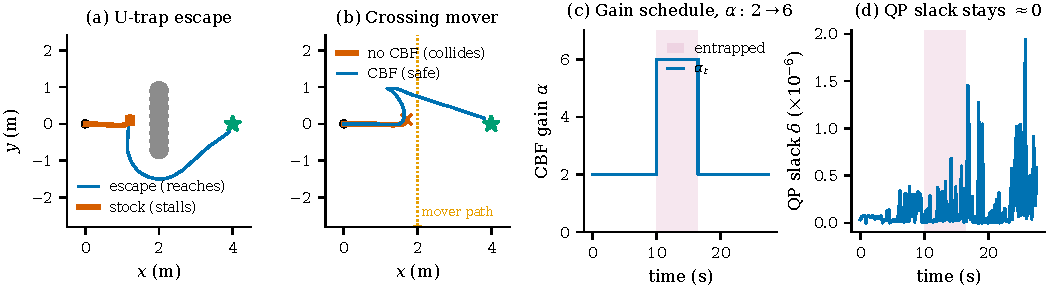
\includegraphics[width=\linewidth]{figures/mechanism.pdf}
\caption{\textbf{Mechanism validation in the 2D mirror} (seed-fixed single runs; \cref{tab:mechanism}). \textbf{(a)}~Stock MPPI stalls at the mouth of a finite wall ($x\approx1.2$\,m) while the detection-and-escape layer rounds it to the goal. \textbf{(b)}~Against a mover crossing the path, the no-CBF controller collides ($\times$) while the look-ahead-point CBF filter keeps the robot clear. \textbf{(c,\,d)}~On the U-trap, the coordinated gain rises from $\alpha_{\mathrm{base}}{=}2$ to $\alpha_{\mathrm{escape}}{=}6$ while entrapped (shaded) and the QP slack stays below $2\times10^{-6}$ throughout: the escape is admitted without relaxing the barrier, close to the slack-free setting that \cref{prop:invariance} assumes. Regenerated as vector graphics by \texttt{scripts/make\_figures.py}.}
\label{fig:mechanism}
\end{figure}

\begin{table}[t]
\centering
\caption{\textbf{Mechanism validation} (single seed-fixed runs of the 2D mirror; 40\,s budget). ``Stalled'' = budget exhausted without progress. Source: \texttt{data/mechanism\_validation.json}, regenerated from \texttt{experiments/prototype/run\_validation.py}.}
\label{tab:mechanism}
\small
\begin{tabular}{llccccc}
\toprule
Scenario & Configuration & Reached & Collided & Time (s) & Min.\ clear.\ (m) & $\max_t\alpha_t$ \\
\midrule
U-trap & stock MPPI (A) & no (stalled) & no & -- & 0.33 & 2 \\
U-trap & escape (C) & yes & no & 27.7 & 0.32 & 2 \\
Crossing mover & escape, no CBF (C) & no & yes & -- & $-$0.00 & 2 \\
Crossing mover & \sname{} (F) & yes & no & 18.6 & 0.01 & 6 \\
U-trap & \sname{} (F) & yes & no & 27.7 & 0.32 & 6 \\
U-trap + mover & independent (E) & yes & no & 27.7 & 0.32 & 2 \\
\bottomrule
\end{tabular}
\end{table}


\noindent\textbf{Mechanism Check.} Before measuring rates, we verify that each mechanism does what it is designed to do on three hand-built scenes (\cref{fig:mechanism}, \cref{tab:mechanism}). Stock MPPI stalls in front of a finite wall for the full $40$\,s budget, while the escape layer reaches the goal in $27.7$\,s; against a crossing mover the no-CBF controller collides after $4.7$\,s, while the CBF filter reaches the goal in $18.6$\,s with the minimum clearance never negative; and on the U-trap the coordinated gain rises from $2$ to $6$ while entrapped, with QP slack below $2\times10^{-6}$ throughout, so the escape is admitted without relaxing the barrier (\cref{prop:invariance}). In these benign scenes the coordinated and independent variants are both safe and equally fast ($27.7$\,s, $0.32$\,m clearance), so they cannot separate the two; the randomized benchmark below is the quantitative test.

\begin{table}[t]
\centering
\caption{\textbf{Main result: success rate} in \% with Wilson 95\% confidence interval, $N=50$ paired scenarios per cell ($1{,}200$ trials of the Python 2D mirror, not the Nav2 controller). Best per family in bold. On the two trap families the escape configurations (C, E, F) separate from stock (A), CBF only (D) and the no-gap ablation (F$^{-}$), which all stay at $0\%$. Source: \texttt{experiments/results\_2d/summary.csv}.}
\label{tab:main}
\small
\begin{tabular}{lcccc}
\toprule
Configuration & U-trap & Clutter & Dynamic & Narrow-dyn. \\
\midrule
A\,stock MPPI & 0\,{\scriptsize[0,7]} & 52\,{\scriptsize[39,65]} & 80\,{\scriptsize[67,89]} & 0\,{\scriptsize[0,7]} \\
C\,escape only & \textbf{90}\,{\scriptsize[79,96]} & \textbf{62}\,{\scriptsize[48,74]} & 76\,{\scriptsize[63,86]} & \textbf{78}\,{\scriptsize[65,87]} \\
D\,CBF only & 0\,{\scriptsize[0,7]} & 52\,{\scriptsize[39,65]} & 82\,{\scriptsize[69,90]} & 0\,{\scriptsize[0,7]} \\
E\,escape+CBF (indep.) & 88\,{\scriptsize[76,94]} & \textbf{62}\,{\scriptsize[48,74]} & 78\,{\scriptsize[65,87]} & 64\,{\scriptsize[50,76]} \\
\textbf{F\,\sname{} (coord.)} & 88\,{\scriptsize[76,94]} & \textbf{62}\,{\scriptsize[48,74]} & 78\,{\scriptsize[65,87]} & 62\,{\scriptsize[48,74]} \\
F$^{-}$\,F without gap search & 0\,{\scriptsize[0,7]} & 52\,{\scriptsize[39,65]} & \textbf{84}\,{\scriptsize[71,92]} & 0\,{\scriptsize[0,7]} \\
\bottomrule
\end{tabular}
\end{table}

\begin{table}[t]
\centering
\caption{\textbf{Paired contrasts against F} (McNemar on success, Holm-adjusted within each family of 16 tests). $b$ = trials the baseline solves and F does not; $c$ = the reverse. $^{*}$ marks $p_{\mathrm{adj}}<0.05$. The escape contrast (A$\to$F) is decisive on both trap families; the coordination contrast (E$\to$F) is null everywhere. Source: \texttt{experiments/results\_2d/stats.json}.}
\label{tab:contrasts}
\small
\begin{tabular}{lcccccc}
\toprule
 & \multicolumn{2}{c}{Escape (A$\to$F)} & \multicolumn{2}{c}{CBF cost (C$\to$F)} & \multicolumn{2}{c}{Coordination (E$\to$F)} \\
\cmidrule(lr){2-3}\cmidrule(lr){4-5}\cmidrule(lr){6-7}
Family & $b/c$ & $p_{\mathrm{adj}}$ & $b/c$ & $p_{\mathrm{adj}}$ & $b/c$ & $p_{\mathrm{adj}}$ \\
\midrule
U-trap & 0/44 & $1.4\!\times\!10^{-9}$$^{*}$ & 1/0 & 1 & 0/0 & 1 \\
Clutter & 0/5 & 1 & 0/0 & 1 & 0/0 & 1 \\
Dynamic & 3/2 & 1 & 1/2 & 1 & 0/0 & 1 \\
Narrow-dyn. & 0/31 & $1.1\!\times\!10^{-6}$$^{*}$ & 8/0 & 0.109 & 1/0 & 1 \\
\bottomrule
\end{tabular}
\end{table}


\noindent\textbf{The Escape Layer Is the Measured Contribution.} On both trap families the effect is decisive and survives Holm correction (\cref{tab:main,tab:contrasts}). Success rises from $0\%$, where stock A, CBF-only D and no-gap F$^{-}$ all time out in the pocket, to $88$--$90\%$ on U-trap (44 of 50 discordant pairs in F's favour, $p_{\mathrm{adj}}=1.4\times10^{-9}$) and to $62$--$78\%$ on narrow-dynamic (31 of 50, $p_{\mathrm{adj}}=1.1\times10^{-6}$). On clutter the escape adds $10$ percentage points ($52\%\to62\%$, not significant after correction) at the cost of about $2.4$\,s longer mean time-to-goal over successful trials ($15.2$\,s $\to$ $17.7$\,s; \cref{tab:full}). On the pure dynamic family, which contains no trap, it is appropriately neutral (A$\to$F: $b/c=3/2$, $p_{\mathrm{adj}}=1$). \Cref{fig:success} shows the full per-family picture, including collision and timeout rates.

\begin{figure}[t]
\centering
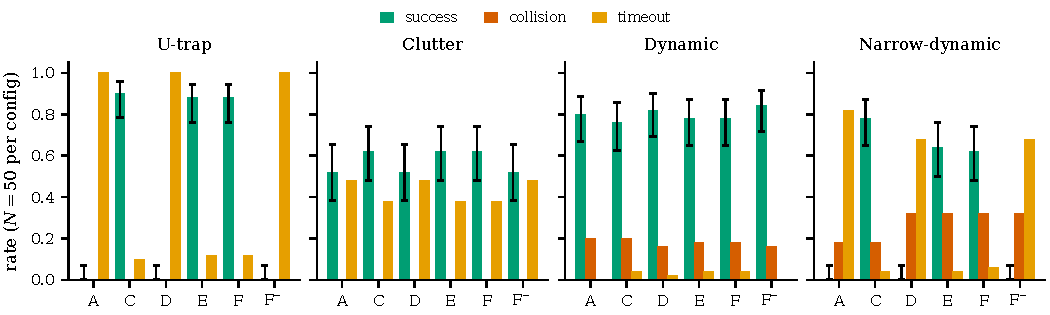
\includegraphics[width=\linewidth]{figures/success_bars.pdf}
\caption{\textbf{Outcome rates per family} across configurations A--F$^{-}$ ($N=50$ each; Wilson 95\% intervals on success). On the trap families (U-trap, narrow-dynamic) the escape configurations C, E and F separate from A, D and F$^{-}$, which time out at $0\%$ success. Plotted directly from \texttt{experiments/results\_2d/summary.csv}.}
\label{fig:success}
\end{figure}


\subsection{Ablation Studies}\label{sec:ablation}

\noindent\textbf{The Gap Search Is Load-Bearing.} F$^{-}$, which keeps the entrapment detector, the APF repulsion and the gain modulation but drops the gap search, scores $0\%$ on both trap families (\cref{tab:main}), identical to stock MPPI. Detection-and-switch escapes only \emph{with} the free-space gap subgoal: repulsion and gain modulation without a routed opening do not escape.

\noindent\textbf{Escape--Safety Coordination Is Null in This Regime.} The contrast that bears on the coordination contribution is E (independent) versus F (coordinated): identical mechanisms that differ only in whether the CBF gain follows the escape phase. Across all $200$ paired scenarios this contrast is null (\cref{tab:contrasts}, \cref{fig:evsf}): the discordant counts are $0/0$, $0/0$, $0/0$ and $1/0$, McNemar $p=1$ in every family, and every continuous effect size (Cliff's $\delta$) satisfies $|\delta|\le0.032$. The gain does engage as designed ($\max_t\alpha_t=6$ during escape, TTC override active). The per-trial slack telemetry (\cref{tab:slack}) locates where the barrier actually works. On the mover-free families the dynamic-obstacle CBF sees no obstacle at all: slack is zero in every trial, E and F issue identical commands, and the null there is structural. On narrow-dynamic the barrier \emph{does} engage and even relaxes, with nonzero slack in $34$ of $50$ trials for E and F ($26$ for D and F$^{-}$, maximum $0.47$), and on dynamic in $47$--$48$ of $50$ (maximum $0.015$); yet E and F still do not differ. The correct reading is therefore not that the barrier never binds, but that the \emph{outcomes are insensitive to the $\alpha$ schedule}: where the barrier is quiescent the two configurations coincide exactly, and where it is active both gains admit escapes whose outcomes are indistinguishable at $N=50$. In this benchmark the coordination produces no measurable outcome difference over independent escape+CBF. This is consistent with, and delimits, \cref{prop:invariance}: coordination is a certified-safe mechanism, not, in these scenarios, an outcome improvement.

\begin{figure}[t]
\centering
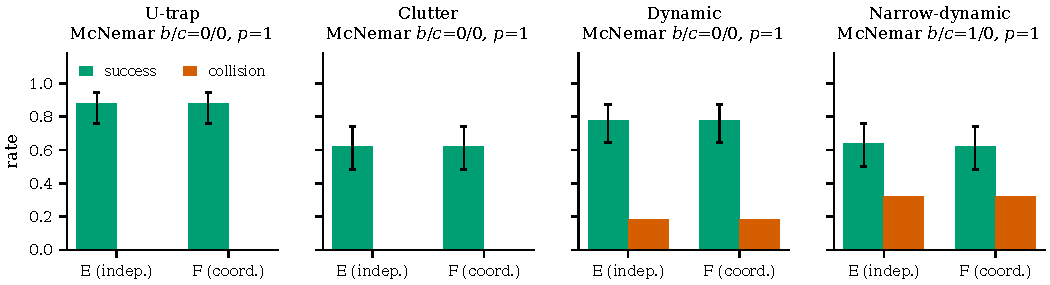
\includegraphics[width=\linewidth]{figures/e_vs_f.pdf}
\caption{\textbf{The coordination contrast is null.} Independent escape+CBF (E) versus coordinated \sname{} (F) per family, with the paired McNemar discordant counts and raw $p$-values from \texttt{experiments/results\_2d/stats.json}. The two are indistinguishable in every family.}
\label{fig:evsf}
\end{figure}


\noindent\textbf{What the CBF Changes.} Against body-grazing crossers (dynamic) the look-ahead-point filter leaves the collision rate essentially unchanged ($20\%$ for A versus $16$--$18\%$ with a CBF; descriptive, since the committed analysis carries no paired collision test). In the cramped narrow-dynamic pocket, the CBF configurations show a \emph{higher} collision rate than their no-CBF counterparts ($18\%\to32\%$, descriptive) and lose about $16$ points of success (C $78\%$ versus F $62\%$; McNemar $b/c=8/0$, raw $p=0.008$, $p_{\mathrm{adj}}=0.109$), which is directionally consistent though not significant after correction at $N=50$. We attribute both to the braking fallback and the point certificate and discuss them as limitations in \cref{sec:discussion}.

\subsection{Live Nav2 and Gazebo Integration}\label{sec:live}

We deployed \sname{} in a complete live stack: ROS~2 Jazzy, Nav2 (AMCL, costmaps, NavFn, behaviour-tree navigator, recovery, collision monitor) and the Gazebo \code{tb3_sandbox} world. The committed launch logs and trial telemetry confirm that the controller and the \code{EscapeCritic} load and activate from the critics list, that the controller produces velocity commands of the same form as stock MPPI, and that the lifecycle reaches the active state and sustains multi-minute drives on a U-trap testbed without a crash or collision after the fix below. The goal was not reached: the committed telemetry records STUCK at $254.5$\,s and TIMEOUT at $299.8$\,s, both collision-free, under the host constraints of \cref{sec:setup}. The escape-injection path has also run live: its first live activation exposed the ABI fault below, and the tensor shapes captured from that event are committed as a regression test, while the controller and critic now log every detection and injection transition for auditability. A sustained live entrapment-and-escape demonstration remains confounded by the host artefacts and is deferred to a GPU workstation. Three faults surfaced that only a live stack reveals:
\begin{itemize}
    \item \emph{Static walls in the CBF.} Feeding every lethal cluster, walls included, into the CBF makes the barrier infeasible everywhere and freezes the robot; scoping the CBF to moving, body-sized obstacles \eqref{eq:track} fixes it.
    \item \emph{Compute budget.} The per-cycle budget must match the host (horizon preserved, rate and batch reduced), or the loop misses its rate and the optimizer diverges.
    \item \emph{xtensor ABI mismatch.} The installed \code{libmppi_controller.so} is compiled with \code{XTENSOR_USE_XSIMD} and AVX2 (an aligned-allocator element type), whereas our plugin used the default allocator. Because the critic tensors cross the pluginlib boundary by reference, the first \code{EscapeCritic} write to \code{data.costs} violated the one-definition rule and crashed the whole Nav2 process on the first live escape injection. Unit tests could not catch it, since they compile every translation unit with one flag set, and earlier live runs had never triggered entrapment. Compiling the critic with the installed headers' flags, per target because a global AVX2 switch breaks the separately built OSQP--Eigen boundary, fixes it, and a regression test replays the injection with the live tensor shapes.
\end{itemize}
This is the class of fault a Nav2-native deployment exposes and that a standalone node or a pure 2D study cannot.

\section{Discussion and Limitations}\label{sec:discussion}

\noindent\textbf{Where Should Coordination Matter?} The null E-versus-F result does not contradict the design; it bounds where the design can pay off. An outcome-level benefit requires a regime in which the choice of $\alpha$ changes \emph{which} escape manoeuvres are admitted at outcome-deciding moments: faster or persistent movers, tighter margins, or a dynamic gap the escape route must thread while the barrier is active. Our generator's pedestrian-like movers produce barrier engagement (\cref{tab:slack}) but not that sensitivity. Constructing and measuring such a regime is future work, and we claim no coordination benefit we have not measured.

\noindent\textbf{Cost Analysis.} We do not report per-cycle compute. The benchmark runs a Python mirror whose timings say nothing about the C++ plugin, and the compute telemetry of the committed live pilot trials is empty ($n=0$ samples), so any figure would be unsupported. The QP adds one small solve per cycle whose size grows with the obstacle budget $N_{\mathrm{obs}}$ (capped by clearance pruning), and the escape terms are evaluated only while entrapped; measuring their cost on a real-time-capable host belongs to the full-scale benchmark.

\noindent\textbf{Deployment Lessons.} The three live faults of \cref{sec:live} share a pattern: each sits on an interface (costmap semantics, the compute budget, the binary interface across the pluginlib boundary) that unit tests with one consistent build configuration and synthetic inputs do not exercise. For controller plugins that write into another library's tensors, we recommend compiling against the installed headers' exact flags and committing a regression test that replays live-captured shapes.

\noindent\textbf{Limitations.} We state the limits of the evidence explicitly.
\begin{itemize}
    \item \emph{Full-scale physics benchmark not run.} The quantitative comparison is the 2D mirror, not the live controller. The specified full-scale protocol, an identical Nav2 stack and differential robot across BARN \citep{barn,barn_challenge}, DynaBARN \citep{dynabarn} and HuNavSim \citep{hunavsim} against stock MPPI \citep{nav2,mppi_orig}, DWB \citep{dwa}, RPP \citep{rpp}, TEB \citep{teb}, a DRPA-style always-on escape \citep{drpa_mppi} and a Shield-style CBF-only controller \citep{shield_mppi}, scored by success, collision, time-to-goal, path length, clearance and compute under the same statistics, needs a GPU workstation we did not have. The live entrapment-and-escape reproduction is deferred for the same reason.
    \item \emph{Coordination benefit unmeasured.} The coordination is certified-safe by construction but produced no outcome difference over independent escape+CBF (\cref{sec:ablation}).
    \item \emph{Braking is not a safe fallback when cornered.} In the narrow-dynamic pocket the infeasible-QP fallback ($v=0$) leaves the robot in the path of a sweeping mover, and the CBF configurations collide more often than their no-CBF counterparts ($18\%\to32\%$). A cornered robot needs an evasive fallback, not a stop.
    \item \emph{Look-ahead point versus full body.} \Cref{prop:invariance} certifies the look-ahead point $\mathbf{P}_t$, not the robot body. Body safety is approximate: $L\approx r$ places $\mathbf{P}_t$ at the leading edge, and the costmap critic and \code{collision_monitor} cover the residual. Full-body certification would inflate the margin by $L$, which we avoid because it over-constrains sub-metre gaps. The gap is visible in the data: body-grazing crossers still collide at $16$--$18\%$ with the filter.
    \item \emph{Sampled-data and slack caveats.} Invariance between samples is assumed (\cref{as:intersample}), not proven, and the shared slack couples the rows of one solve; we report slack usage instead of an unconditional certificate.
    \item \emph{Constant-velocity tracker.} The obstacle model evaluated here is a constant-velocity baseline that mispredicts turning or accelerating agents and does not quantify its uncertainty. The released controller has since added occupancy-persistence static/dynamic classification, least-squares horizon prediction and an online conformal radius; these belong to follow-up work, and none of them is present in the 2D mirror behind every quantitative result reported here.
    \item \emph{Other approximations.} The TTC is a one-dimensional closing-speed estimate that can induce over-rotation in tight spaces, and localization jumps in symmetric or narrow maps can perturb the progress signal.
\end{itemize}

\section{Conclusion}\label{sec:conclusion}

We presented \sname, which packages local-minima escape and control-barrier-function safety, usually studied apart, in a single deployable Nav2 controller: one entrapment signal drives both a sampling-time escape critic and an output-time CBF filter, and a coordinated gain lets the robot escape while a forward-invariance argument keeps the escape certified-safe. On a randomized, paired $1{,}200$-trial 2D benchmark, the online detection-and-escape layer is the decisive contribution, raising success from $0\%$ to $88$--$90\%$ on the U-trap family and from $0\%$ to $62$--$78\%$ on the narrow-dynamic family, with the free-space gap search load-bearing, whereas the coordination is statistically indistinguishable from independent escape+CBF in the regimes we could test. The controller loads, activates and runs in a full ROS~2 Jazzy, Nav2 and Gazebo stack, where three integration faults surfaced that only a live deployment reveals. The remaining step is the full-scale physics benchmark on a real-time-capable GPU host.

\bibliography{main}
\clearpage
\appendix
\section{Reproduction}\label{app:repro}

All paths are relative to the code release (\url{https://github.com/kjungmo/se-mppi-nav2}, Apache-2.0).

\noindent\textbf{Software.} ROS~2 Jazzy, Nav2 and Gazebo are installed through RoboStack (conda channels \code{robostack-jazzy} and \code{conda-forge}) by \code{scripts/setup_ros2_env.sh}, which also installs \code{osqp-eigen} and \code{eigen} for the CBF-QP and a compiler toolchain, so the build does not depend on the host OS version.

\noindent\textbf{Benchmark regeneration.} Every benchmark number is generated from the committed per-trial file by committed scripts. The committed data use $N=50$:
{\small
\begin{verbatim}
export MAMBA_ROOT_PREFIX=$HOME/micromamba
micromamba run -n ros2 python3 -m experiments.benchmark2d.runner \
    --families utrap clutter dynamic narrowdyn -n 50 --workers 6 --max-steps 400
micromamba run -n ros2 python3 -m experiments.benchmark2d.report
\end{verbatim}
}
\noindent The figures and tables of this paper are regenerated from those outputs, and the mechanism runs of \cref{tab:mechanism} are re-executed, by
{\small
\begin{verbatim}
micromamba run -n ros2 python3 docs/papers/arxiv_ref/scripts/make_figures.py
python3 docs/papers/arxiv_ref/scripts/make_tables.py
python3 scripts/check_paper_numbers.py --arxiv
\end{verbatim}
}

\noindent\textbf{Scenarios and seeds.} Seeds $0$--$49$ per family; the generators in \code{experiments/benchmark2d/scenarios.py} seed \code{numpy} generators with a per-family offset plus the trial seed ($10^{6}$ U-trap, $2\times10^{6}$ clutter, $3\times10^{6}$ dynamic, $4\times10^{6}$ narrow-dynamic), and the MPPI noise stream uses the same trial seed (\code{experiments/benchmark2d/runner.py}), so every configuration sees identical worlds and rollout noise. The six toggle sets are in \code{experiments/benchmark2d/configs.py}; the overlays for the deferred full-scale protocol are in \code{experiments/configs/ablations.yaml}.

\noindent\textbf{Data.} Raw per-trial data: \code{experiments/results_2d/trials.csv} ($1{,}200$ rows). Aggregates and statistics: \code{summary.csv}, \code{stats.json}, \code{tables.md} in the same directory. Live pilot telemetry and logs: \code{experiments/results_pilot/}. The claim-to-artifact map for this paper is \code{docs/papers/arxiv_ref/NUMBERS.md}.

\section{Parameters}\label{app:params}

\begin{table}[!htbp]
\centering
\caption{\textbf{Parameters.} Released-controller defaults come from the package's parameter file and parameter getters; 2D-mirror values from the prototype primitives and the benchmark rollout (\cref{app:repro,app:mirror}).}
\label{tab:params}
\footnotesize
\setlength{\tabcolsep}{4pt}
\begin{tabular}{llcc}
\toprule
Symbol & Meaning & Released controller & 2D mirror \\
\midrule
$T,\ \Delta t$ & MPPI horizon steps, step (s) & 56, 0.05 & 25, 0.1 \\
$K$ & rollouts per cycle & 1000 & 600 \\
$\lambda$ & MPPI temperature & 0.3 & 0.3 \\
$\Sigma^{1/2}$ & sampling std.\ of $(v,\omega)$ & (0.2, 0.4) & (0.25, 0.6) \\
$\mathcal{U}$ & $v\in[v_{\min},v_{\max}]$, $|\omega|\le\omega_{\max}$ & $[-0.35, 0.5]$, 1.9 & $[-0.35, 0.5]$, 1.9 \\
$W$ & entrapment stall window (cycles) & 30 & 15 \\
$\epsilon_{\mathrm{goal}}$ & entrapment suppression radius (m) & 0.5 & -- \\
$d_0,\ \eta$ & APF influence distance (m), gain & 0.6, 1.0 & 0.8, 0.3 \\
$N_r,\ r_{\max},\ r_{\min}$ & gap rays, ray range (m), min.\ clearance (m) & 36, 2.0, 0.6 & 72, 3.0, 2.4 \\
$w_g$ & gap-attraction weight & 4.0 & subgoal (\cref{app:mirror}) \\
$L$ & look-ahead distance (m) & 0.2 & 0.2 \\
$r,\ m$ & robot radius (m), safety margin (m) & 0.225 (logged), 0.05 & 0.22, 0.05 \\
$\rho$ & QP slack weight & $10^{3}$ & $10^{3}$ \\
$\epsilon_\delta$ & slack threshold for braking & $10^{-3}$ & $10^{-3}$ \\
$N_{\mathrm{obs}}$ & obstacles kept in the QP & 20 & all dynamic \\
$\alpha_{\mathrm{base}},\ \alpha_{\mathrm{escape}}$ & CBF class-$\mathcal{K}$ gains & 2.0, 6.0 & 2.0, 6.0 \\
$\tau$ & TTC override threshold (s) & 1.5 & 1.5 \\
$v_{\mathrm{dyn}},\ R_{\max}$ & CBF admission: min.\ speed (m/s), max.\ radius (m) & 0.1, 1.0 & $\|\mathbf{v}_o\|>0$ \\
\bottomrule
\end{tabular}
\end{table}


\section{Differences Between the 2D Mirror and the Nav2 Controller}\label{app:mirror}

The 2D mirror (\code{experiments/prototype/se_mppi_proto.py}, driven by \code{experiments/benchmark2d/rollout.py}) reuses the controller's formulas but differs in the following documented ways.
\begin{itemize}
    \item \emph{Progress signal.} Without a global path, entrapment is declared when the best distance-to-goal has not improved by $10^{-3}$\,m for $W=15$ cycles, instead of the stall of $k^{\max}_t$ in \eqref{eq:detect}.
    \item \emph{Gap use.} The selected gap bearing places a temporary subgoal $2.5$\,m along the opening, replacing the goal in the MPPI cost while entrapped, in lieu of Nav2's global routing and the critic's $C_{\mathrm{gap}}$ term; the gap choice carries a hysteresis term toward the previous bearing so that symmetric openings do not flip every cycle.
    \item \emph{Geometry.} Obstacles, including walls built from chains of discs, are circles; APF distances and ray lengths are computed analytically against them rather than on a costmap distance field.
    \item \emph{Obstacle knowledge.} The CBF and TTC receive the true positions and velocities of the moving obstacles, so the tracker of \cref{sec:track} is not exercised.
    \item \emph{Costs.} The MPPI cost is a goal-distance, path-progress and obstacle-proximity cost rather than Nav2's critic stack; parameters differ as listed in \cref{tab:params}.
    \item \emph{Mechanism scenes.} \Cref{tab:mechanism} comes from \code{run_validation.py}, whose CBF sees all obstacles, including the static wall discs; the benchmark mirror restricts the CBF to movers, as the Nav2 controller does.
\end{itemize}

\section{Extended Results}\label{app:results}

\begin{table}[!htbp]
\centering
\caption{\textbf{Full per-family results} of the Python 2D-mirror benchmark ($N=50$ per cell). Rates in \%; time-to-goal and path length are means over successful trials only (\,$\pm$ 95\% CI half-width); minimum clearance is over all trials. Source: \texttt{experiments/results\_2d/summary.csv}.}
\label{tab:full}
\footnotesize
\setlength{\tabcolsep}{4pt}
\begin{tabular}{llcccccc}
\toprule
Family & Config & Succ. & Coll. & Timeout & Time-to-goal (s) & Path (m) & Min.\ clear.\ (m) \\
\midrule
\multirow{6}{*}{U-trap} & A & 0 & 0 & 100 & -- & -- & 0.33\stdv{0.00} \\
 & C & 90 & 0 & 10 & 31.34\stdv{1.36} & 8.12\stdv{0.33} & 0.32\stdv{0.00} \\
 & D & 0 & 0 & 100 & -- & -- & 0.33\stdv{0.00} \\
 & E & 88 & 0 & 12 & 31.20\stdv{1.36} & 8.09\stdv{0.32} & 0.32\stdv{0.00} \\
 & F & 88 & 0 & 12 & 31.20\stdv{1.36} & 8.09\stdv{0.32} & 0.32\stdv{0.00} \\
 & F$^{-}$ & 0 & 0 & 100 & -- & -- & 0.33\stdv{0.00} \\
\midrule
\multirow{6}{*}{Clutter} & A & 52 & 0 & 48 & 15.23\stdv{0.49} & 5.81\stdv{0.17} & 0.36\stdv{0.02} \\
 & C & 62 & 0 & 38 & 17.67\stdv{2.11} & 6.14\stdv{0.32} & 0.35\stdv{0.02} \\
 & D & 52 & 0 & 48 & 15.23\stdv{0.49} & 5.81\stdv{0.17} & 0.36\stdv{0.02} \\
 & E & 62 & 0 & 38 & 17.67\stdv{2.11} & 6.14\stdv{0.32} & 0.35\stdv{0.02} \\
 & F & 62 & 0 & 38 & 17.67\stdv{2.11} & 6.14\stdv{0.32} & 0.35\stdv{0.02} \\
 & F$^{-}$ & 52 & 0 & 48 & 15.23\stdv{0.49} & 5.81\stdv{0.17} & 0.36\stdv{0.02} \\
\midrule
\multirow{6}{*}{Dynamic} & A & 80 & 20 & 0 & 22.48\stdv{1.44} & 7.99\stdv{0.55} & 0.12\stdv{0.03} \\
 & C & 76 & 20 & 4 & 21.87\stdv{1.36} & 7.75\stdv{0.53} & 0.13\stdv{0.03} \\
 & D & 82 & 16 & 2 & 22.74\stdv{1.52} & 8.02\stdv{0.65} & 0.13\stdv{0.03} \\
 & E & 78 & 18 & 4 & 21.77\stdv{1.25} & 7.56\stdv{0.47} & 0.13\stdv{0.03} \\
 & F & 78 & 18 & 4 & 21.78\stdv{1.25} & 7.57\stdv{0.47} & 0.13\stdv{0.03} \\
 & F$^{-}$ & 84 & 16 & 0 & 23.01\stdv{1.66} & 8.14\stdv{0.68} & 0.13\stdv{0.03} \\
\midrule
\multirow{6}{*}{Narrow-dyn.} & A & 0 & 18 & 82 & -- & -- & 0.22\stdv{0.04} \\
 & C & 78 & 18 & 4 & 30.52\stdv{1.30} & 8.33\stdv{0.44} & 0.21\stdv{0.04} \\
 & D & 0 & 32 & 68 & -- & -- & 0.19\stdv{0.04} \\
 & E & 64 & 32 & 4 & 30.55\stdv{1.50} & 8.24\stdv{0.55} & 0.18\stdv{0.04} \\
 & F & 62 & 32 & 6 & 30.36\stdv{1.51} & 8.11\stdv{0.50} & 0.18\stdv{0.04} \\
 & F$^{-}$ & 0 & 32 & 68 & -- & -- & 0.19\stdv{0.04} \\
\bottomrule
\end{tabular}
\end{table}

\begin{table}[!htbp]
\centering
\caption{\textbf{CBF slack usage.} Trials (of 50) in which the QP relaxed a barrier row at least once, and the largest per-trial \texttt{slack\_max}. Configurations without a CBF (A, C) are zero by construction; on the mover-free families the CBF sees no obstacle. Source: \texttt{experiments/results\_2d/stats.json} (\texttt{slack\_usage}).}
\label{tab:slack}
\small
\begin{tabular}{lcccccc}
\toprule
Family & A & C & D & E & F & F$^{-}$ \\
\midrule
U-trap & 0 & 0 & 0 & 0 & 0 & 0 \\
Clutter & 0 & 0 & 0 & 0 & 0 & 0 \\
Dynamic & 0 & 0 & 47 (0.015) & 48 (0.015) & 48 (0.015) & 47 (0.015) \\
Narrow-dyn. & 0 & 0 & 26 (0.469) & 34 (0.469) & 34 (0.469) & 26 (0.469) \\
\bottomrule
\end{tabular}
\end{table}


\Cref{tab:full} lists every configuration and family of the benchmark, and \cref{tab:slack} the slack usage behind the discussion of \cref{sec:coord,sec:ablation}. Configurations E and F coincide exactly on U-trap and clutter because the CBF sees no obstacle in those mover-free families, so the gain schedule is irrelevant there.

\section{Notation}\label{app:notation}

\begin{table}[!htbp]
\centering
\caption{\textbf{Notation.}}
\label{tab:notation}
\small
\begin{tabular}{ll}
\toprule
Symbol & Meaning \\
\midrule
$\mathbf{x}_t=(x_t,y_t,\theta_t)$, $\mathbf{p}_t$ & robot pose, robot position \\
$\mathbf{u}_t=(v_t,\omega_t)$, $\mathcal{U}$ & control (linear, angular velocity), admissible box \\
$\sigma=(\sigma_1,\dots,\sigma_M)$ & global path from the Nav2 planner \\
$k_t,\ k^{\max}_t$ & nearest and furthest-reached path index \\
$s_t,\ W,\ e_t$ & stall counter, stall window, entrapment flag \\
$\mathcal{O}_t$; $\mathbf{p}_o, R_o, \mathbf{v}_o$ & tracked dynamic obstacles; position, radius, velocity \\
$\mathbf{P}_t,\ L,\ G(\theta)$ & look-ahead point, its offset, its Jacobian \\
$h_o,\ R^{\mathrm{eff}}_o$ & barrier for obstacle $o$, effective radius $r+R_o+m$ \\
$\alpha_t$; $\alpha_{\mathrm{base}},\alpha_{\mathrm{escape}}$ & class-$\mathcal{K}$ gain; its two scheduled values \\
$\delta,\ \rho,\ \epsilon_\delta$ & QP slack, slack weight, braking threshold \\
$\mathrm{TTC}_t,\ \tau$ & minimum time-to-collision, override threshold \\
$S^k,\ w^k,\ \lambda$ & rollout cost, softmax weight, temperature \\
$C_{\mathrm{apf}},\ C_{\mathrm{gap}}$ & escape costs (repulsion, gap attraction) \\
$\psi^\star$ & bearing of the selected free-space gap \\
\bottomrule
\end{tabular}
\end{table}


\end{document}
